%!TEX root = ../main.tex
%Motor data object: 4600h. includes motor slip frequency (not relevant), currents, voltages and temperature of heatsink. Don't know yet what the subindices are.
%It is possible to map them to Process Data Object for fixed time updates. It doesn't say anywhere what update rate, we can achieve.
%I've gotten a good amount of data from Karsten.

%This section assumes that CANOpen has been adequately explained beforehand

\paragraph*{Physical Connection}\label{sub:sevcon_physical_connection}~\\
\todo[inline]{Mikkel: Something about sevcon that I don't know where to put??}
The Sevcon utilizes high speed CAN bus for data transfer, and adheres to ISO11898-2.
As such it is recommended to use twisted pair wires with cross section area ranging from $0.5 \si{\milli \meter \squared}$ to $1.5 \si{\milli \meter \squared}$, and terminating the Zybo end with $120 \si{\ohm}$.
On the Sevcon, this can be done by shorting pins 2 and 24, to utilize an internal termination resistor.
There are two CAN interfaces: Pins 13(+) and 24(-) are used for configuration, and pins 16(+) and 27(-) are used to interface with other CAN devices.
The 35 pin connector is shown below for reference:

\begin{figure}[h]
	\centering
	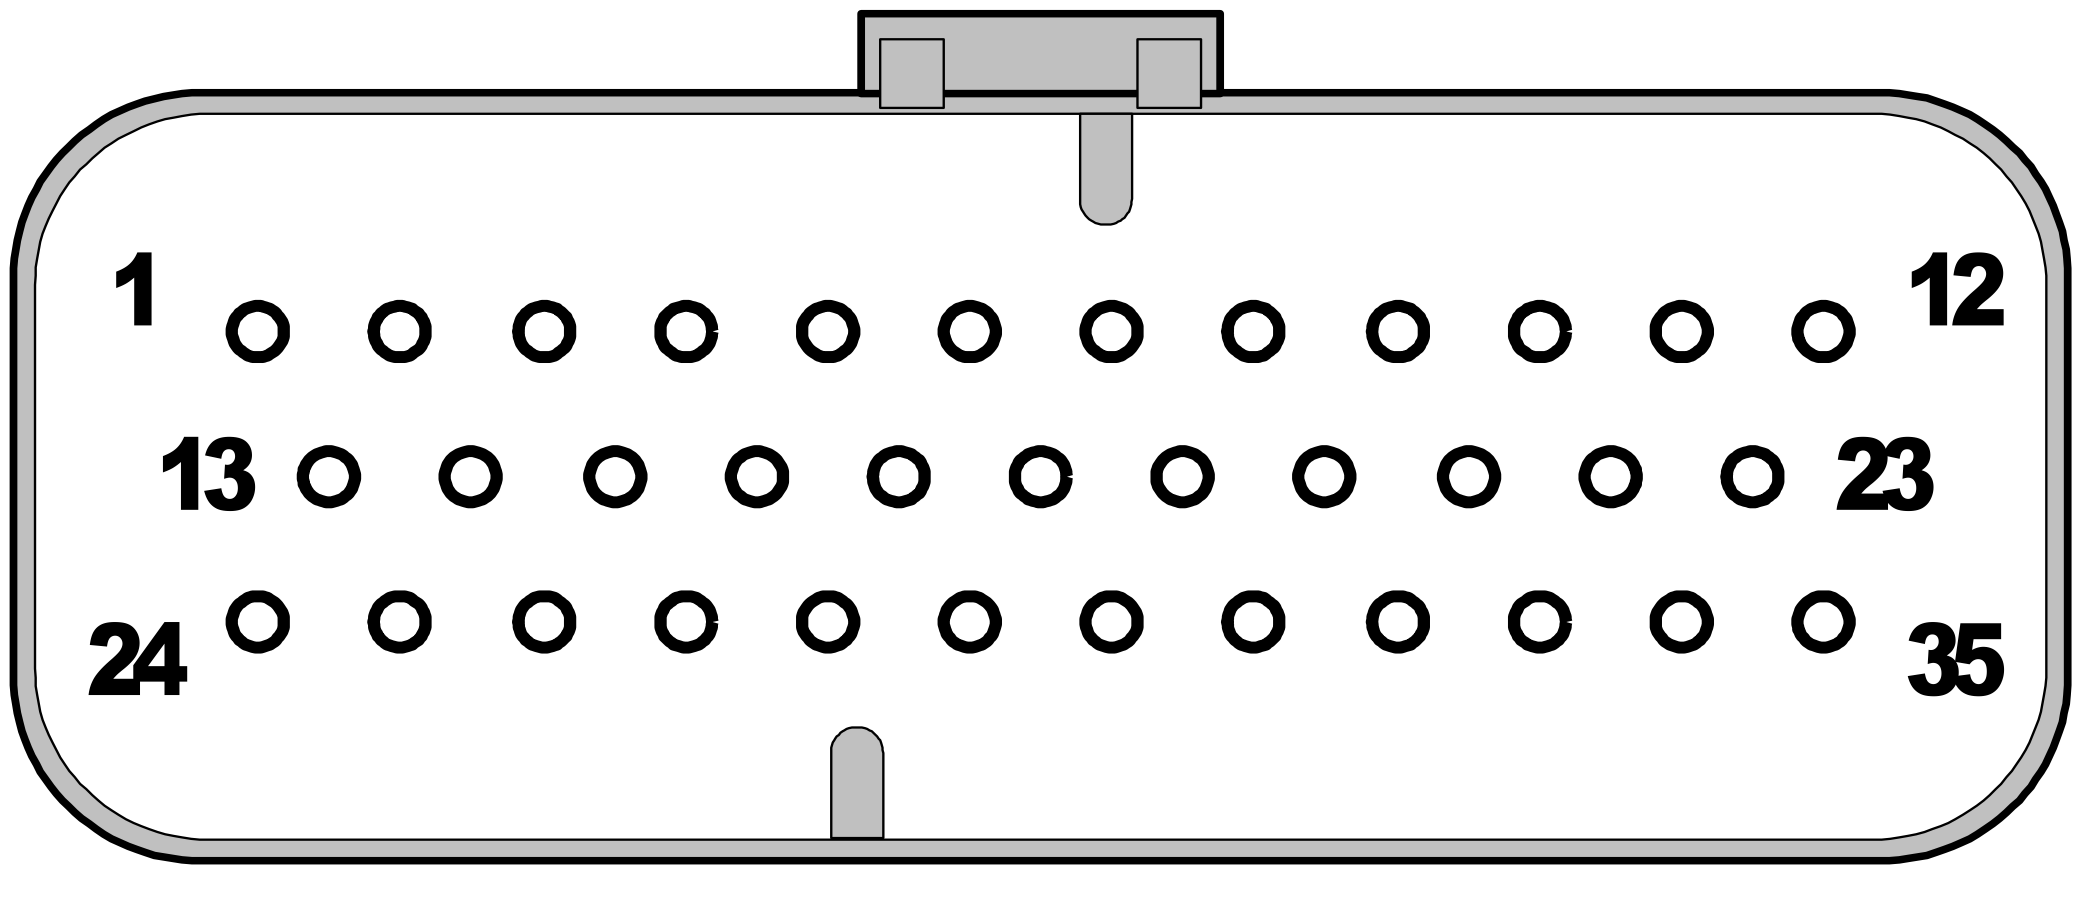
\includegraphics[width = 0.6\linewidth]{graphics/35_pin_dsub}
	\caption{The 35 pin AMPSeal connector used to interface with the Sevcon}
	\label{fig:35_pin_dsub}
\end{figure}

\paragraph*{CANOpen Object Dictionary}\label{sub:sevcon_object_dictionary}~\\
Because the sevcon is so general purpose, its object dictionary is very large, and holds a lot of objects that are completely irrelevant for this particular setup, such as motor slip, and speed control parameters. 
The object directory is documented in a 1400+ Excel file. 
Some objects of interest are:

\begin{table}
	\centering
	\begin{tabular}{| c | c | c | c |}
		\hline
		Parameters & Address & Read/Write & Map to PDO \\ % Excel line
		\hline
		Measured Id & 4600h-7 & Read & Yes \\ %981
		Measured Iq & 4600h-8 & Read & Yes \\ %982
		Target Id & 4600h-5 & Read & Yes \\ %979
		Target Iq & 4600h-6 & Read & Yes \\ %980
		Encoder setup & 4630h-1 to -19 & RW & No \\%1129
		Encoder Read-out & 4630h-9 to -12 & Read & Yes \\ %1137
		Throttle value & 2620h & Read & Yes \\ %330
		Velocity & 606Ch & Read & Yes \\ %1378
		Motor setup & 6072h to 6083h & RW & No \\ %1380	
		\hline	
	\end{tabular}
	\caption{List of some of the parameters readable and writeable through CANOpen}
	\label{tab:parameters_of_interest}
\end{table}

Map to PDO: Can be read at a fixed time interval, so good for monitoring
It does not produce Ia, Ib, Ic. and it does not produce the absolute electrical position, so we'll have to calculate that on the zybo from the sin/cosine values in objets 4630h-9 to -12

